\documentclass{neu_handout}
\usepackage{url}
\usepackage{amssymb}
\usepackage{amsmath}
\usepackage{marvosym}
\usepackage{graphicx}
\usepackage[pdftex]{graphicx}
\usepackage{subfigure}
\graphicspath{ {images/} }
\everymath{\displaystyle}

% Professor/Course information
\title{Update 2}
\author{Emily Dutile, Vyshaal Narayanam, Xiwen Song, Yu Tian}
\date{November 2017}
\course{CS6220}{Data Mining Techniques}

\begin{document}
\section*{1 Introduction and Background}
Today we live in a society where businesses are greatly impacted by customer reviews. For some businesses, this can greatly impact their success or failure. Looking to improve the
experience for restaurant owners and customers, we used the Yelp Open Dataset\footnote{\url{https://www.yelp.com/dataset}} that is filled with restaurant reviews of diverse content and topics, along with how a customers experience was positively or negatively impacted. Through the implementation of several data mining and text mining techniques, we can better understand user reviews and gain new insights into neighborhood businesses. In this project we mine a copious amount of Yelp restaurant reviews to address the following questions: What topics are discovered frequently in reviews and do they correlate to a positive or negative review? What neighborhoods, if any, have the best selection for a particular cuisine in a certain city? Are there some areas in a city that are more upscale or divey than others? Based upon user reviews in a particular city, can we recommend a particular dish at a top restaurant?
\subsection*{1.1 The Data}
The Yelp SQL dataset contains 4.7 million reviews, 156,000 business, and 12 metropolitan areas. Spanning over 10 years of Yelp reviews and 50 states, including international countries, the dataset provides a countless number of questions to be asked. The schema\footnote{\url{https://www.yelp.com/dataset/documentation/sql}} consists of multiple tables including information about businesses, reviews, users, checkins and tips. Since we are familiar with Boston neighborhoods and its cuisines, we wanted to find a city that we thought may have some of the same characteristics. For example, the North End in Boston is known for its Italian food and South Boston is famous for it's Irish heritage and pubs. Since Boston is not in this dataset, the majority of the project focuses on restaurants in Pittsburgh, PA, due to its relatively similar characteristics. Although it has the neighborhood Bloomfield which is equivalent to our Italian North End, Pittsburgh lacks a Chinatown or Irish filled South Boston. Due to this, we were not overly confident that our clustering algorithms will be able to product great results but they may be successful on other cities.
As seen in Figure 1, Pittsburgh is one of the leading cities with respect to its number of restaurants and has many restaurants within close proximity of one another as seen in Figure 2. The heat map of restaurants in Pittsburgh shows that a lot of the neighborhood restaurants in the center of the city are more popular.
\begin{figure}[h]
\centering
\subfigure[Number of Restaurants by City]
{
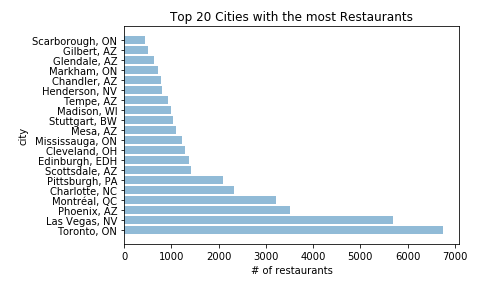
\includegraphics[width=0.47\linewidth]{cities}
}
\subfigure[Heatmap of Pittsburgh restaurants]
{
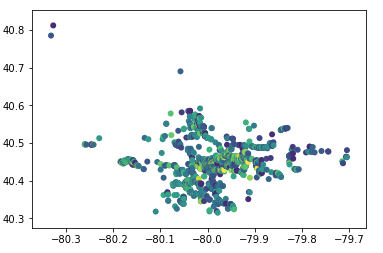
\includegraphics[width=0.4\linewidth]{pa_popular_restaurants}
}
\caption{Graphing and Plotting Pittsburgh}
\end{figure}
Pittsburgh has 2089 restaurants, 53 different neighborhoods, and a diverse cuisine selection (43 different cuisines), which made it an interesting U.S. city to us.
The team setup local databases using PyCharm and MySQLServer in order to run faster queries. For understanding and reproducibility, the project repository and development environment set up instructions can be found on Github\footnote{\url{https://github.com/emily-jean/yelp-data-mining}}.
\subsection*{1.2 Methods}
To answer our questions, we performed data analysis and unsupervised machine learning techniques such as clustering, topic modeling and recommendation. With respect to language processing, tokenization, filtering, lemmatization, and stemming were all used for preprocessing the reviews. To tell if a customer has positive or negative feedback about a restaurant, sentimental analysis was performed in order to see if there is an interesting difference between reviews and ratings although a review is associated with a rating.
\section*{2. Exploratory Analysis}
To better visualize and explore the Pittsburgh neighborhoods a bit more, we discovered the top 10 neighborhoods with the most restaurants. Looking at other outside articles\footnote{url{https://www.thrillist.com/eat/pittsburgh/best-neighborhoods-in-pittsburgh-for-dining-and-eating-out-ranked}}, every one of these neighborhoods are listed as one of the "Best Neighborhoods for Eating" except for Oakland. The second map on the right shows the top 10 neighborhoods with the highest average review count to give some insight as to what neighborhoods are the most popular among Yelp reviewers. In comparison to the Thrillest article, only Lawrenceville, Regent Square, Shadyside, and the Strip District are on their list.

\begin{figure}[h]
\centering
{
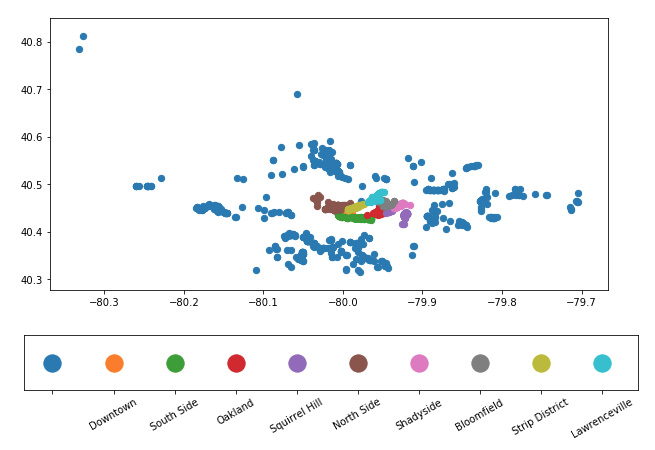
\includegraphics[width=0.47\linewidth]{pitts_hoods_most_restaurants}
}
{
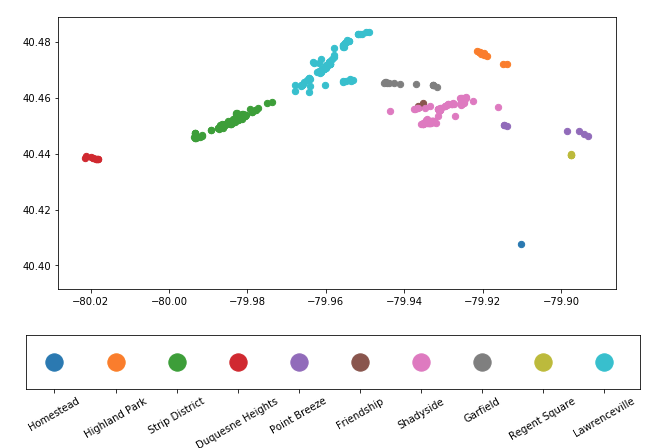
\includegraphics[width=0.47\linewidth]{top_10_most_popular_neighborhoods}
}
\end{figure}

To get started on a deeper exploratory analysis of reviews and ratings, we plotted the distribution of the ratings for all the restaurants in Pittsburgh. From this plot we can see that most restaurants have a rating between 3 and 5. The average rating for Pittsburgh restaurants is 3.51. To gain a deeper insight of the data, we plotted the rating distribution of different cities. Although we are mostly focusing on Pittsburgh, for future analysis we would be interested in comparing differently cities to see if any interesting results arise.

\begin{figure}[h]
\centering
{
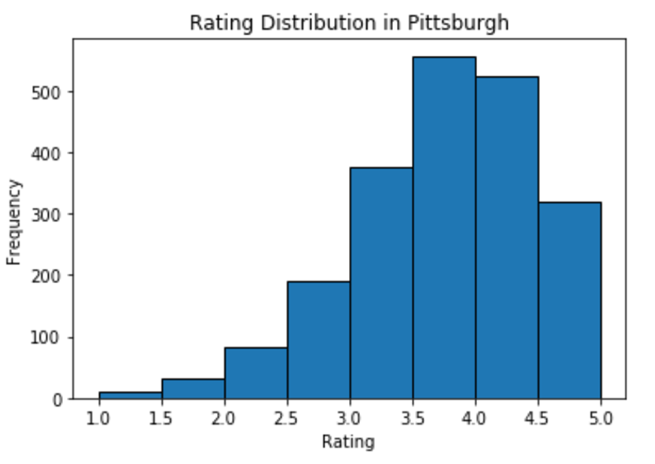
\includegraphics[width=0.4\linewidth]{rating_distribution_in_Pittsburgh}
}
{
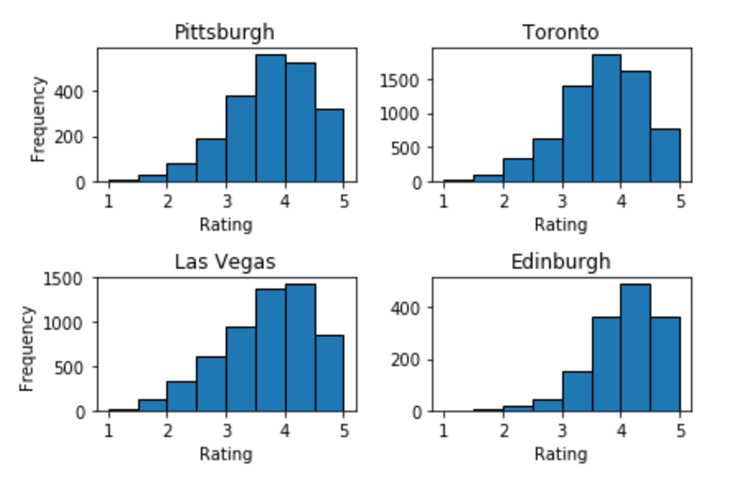
\includegraphics[width=0.4\linewidth]{rating_distribution_vs_countries}
}
\end{figure}

Besides looking at the basic distribution, we plotted the relationship between the average number of reviews and rating levels in Pittsburgh using box plot. Our original belief was that we thought better restaurants should receive more reviews. However, the results showed us that restaurants with a medium rating acquire more reviews. Continuing on the exploration of the relationship between average number of reviews, the average length of review (after tokenization and stemming) and each cuisine, in Pittsburgh in appears that Japanese foods receive the most reviews while Chinese foods receive the least number of reviews. When looking at the length of review, there doesn't appear to be many differences among the variety of cuisines. 

\begin{figure}[h]
\centering
{
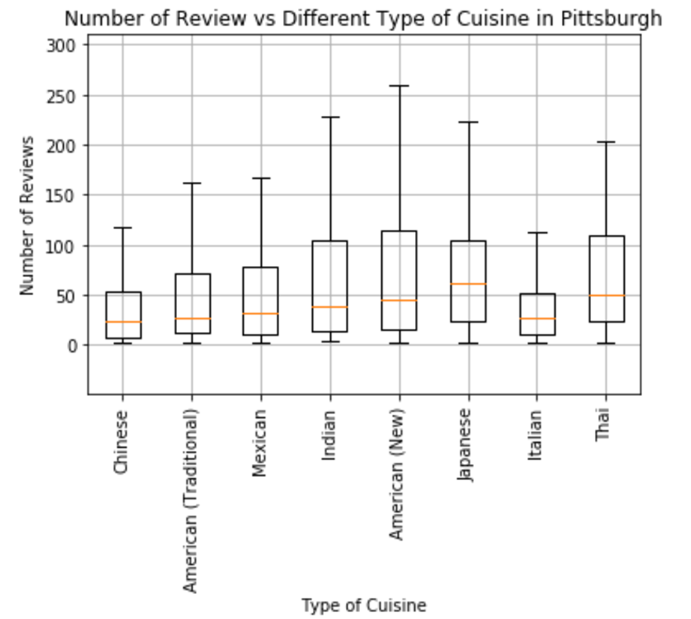
\includegraphics[width=0.35\linewidth]{number_of_review_vs_cuisine}
}
{
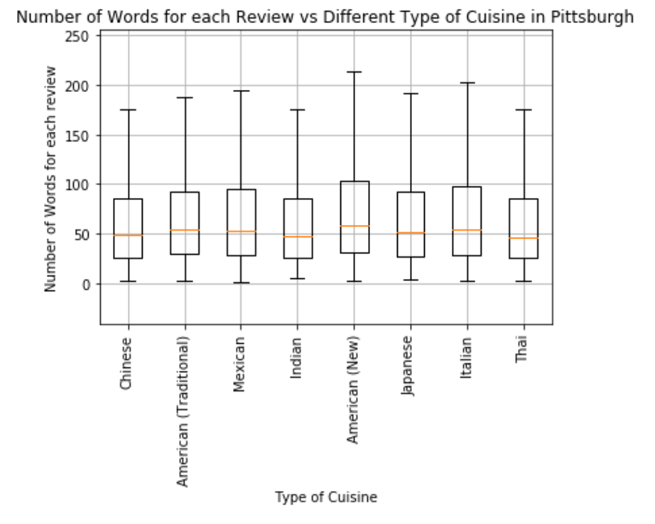
\includegraphics[width=0.4\linewidth]{average_review_length}
}
\end{figure}


Furthermore, to get a better sense on how the contents of a review correlate with the rating, we calculated the ratings for one of the restaurant by performing sentiment analysis on the reviews and then comparing the results with the dataset ratings. Through sentiment analysis, we can determine whether the review is positive or negative. We took a sample dataset of all restaurants in Pittsburgh which have more than 200 reviews to assign our own ratings (there are 109 restaurants in Pittsburgh which satisfy our criteria), and computed the average of the values obtained from sentiment analysis of all the reviews (38,785 reviews) of that restaurant. The sentimental analysis is done using PatternAnalyzer in nltk (textblob is built over nltk). We assigned a weight of +5 for a positive review and -5 for a negative review. These newly derived ratings are compared with the ratings in original dataset as shown in the histogram. We can assume that these reviews are more accurate because we are incorporating negative weights to low star reviews.

\begin{figure}[h]
\centering
{
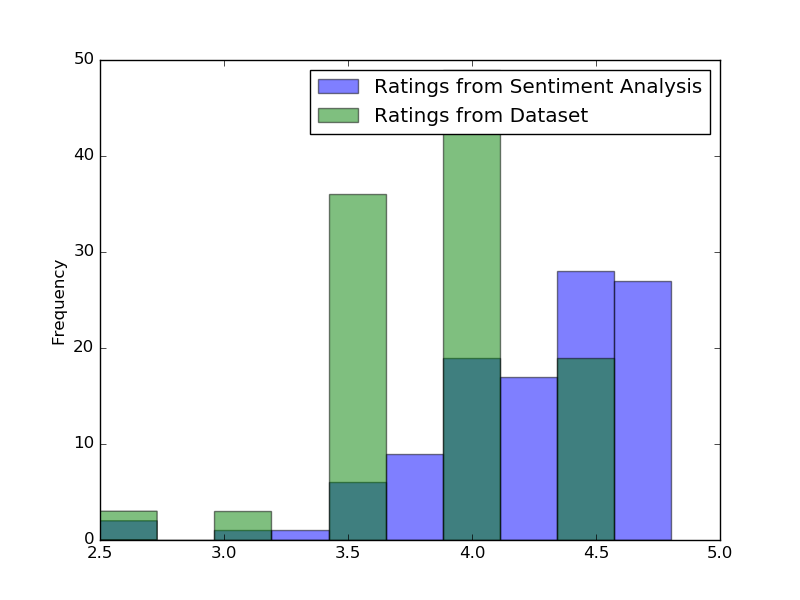
\includegraphics[width=0.4\linewidth]{sentimentanalysis}
}
\end{figure}

Next, we extracted the top 50 keywords from positive and negative reviews. Again taking a sample dataset of all restaurants in Pittsburgh that have more than 200 reviews. There are a total of 38,785 reviews. Data processing techniques such as tokenizing, filtering, stemming and filtering the key words from those reviews were performed. We then calculated 50 most frequent keywords from the negative and positive reviews separately. Negative and positive reviews were distinguished using the polarity obtained in the previous step.
The results are very promising. Few keywords such as "great","good","nice","service" came with high frequency in positive reviews where as words like "bad","good","terrible","poor","great" appeared negative reviews. Common words such as "Pittsburgh", "food", "service", and "place" are present in both positive and negative reviews. One important thing to notice is that "good" and "great" appeared in negative reviews too in a sense that customers are complaining how the food isn't that good/great. The high frequencies of words in positive reviews when compared to negative reviews is because of more number of positive reviews in the corpus.

\begin{figure}[h]
\centering
{
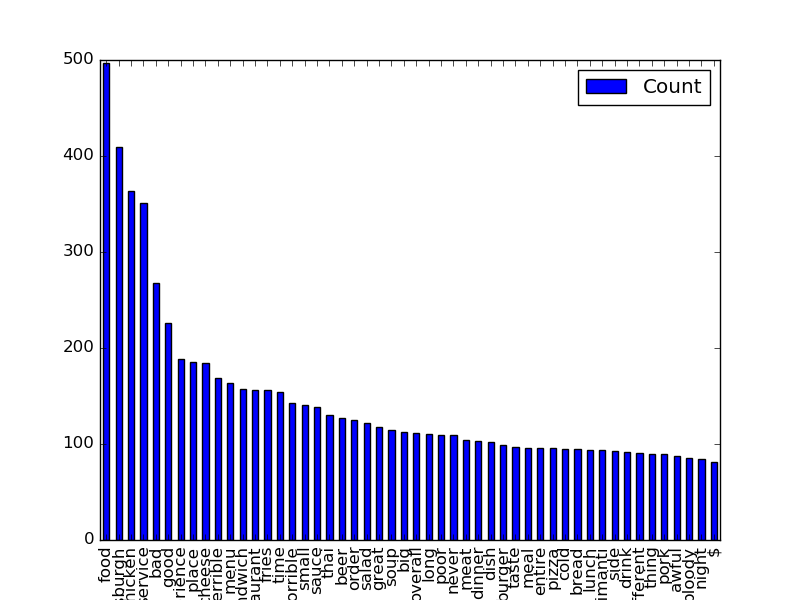
\includegraphics[width=0.4\linewidth]{top50_negativereviews}
}
{
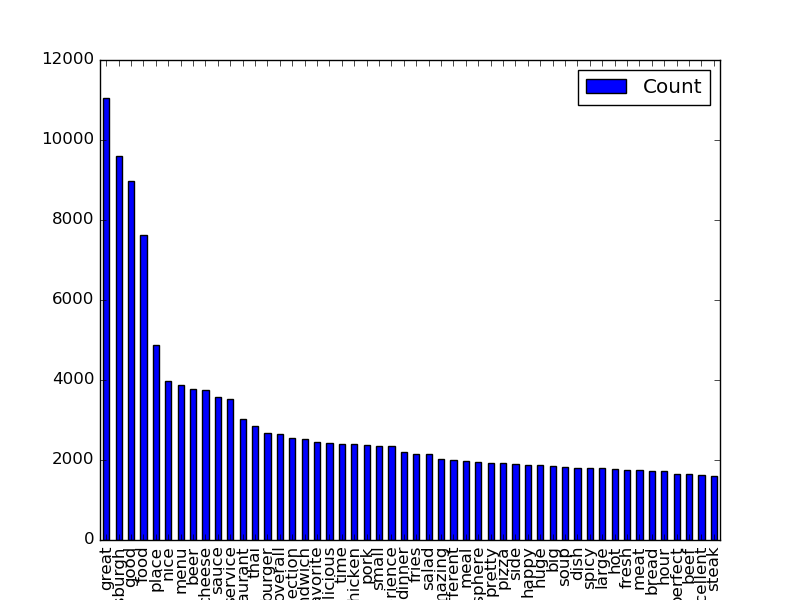
\includegraphics[width=0.4\linewidth]{top50_positivereviews}
}
\end{figure}

Although some of our exploratory analysis focused on one city, we expanded our reviews analysis to 4 different cities with the most reviews (Edinburgh, Toronto, Las Vegas, and Pittsburgh), from 3 different countries. The thought here was that there may be differences between different cities such as the service, or people may have different diction. It's possible that the final cluster may be verified by different external evaluation criteria, so we thought it'd be useful to further explore this area. We plotted the differences of rating habits among the 4 cities based on average rating score for each type of cuisine. Edinburgh has the best rating feedback, relatively speaking, while Toronto seems to be lacking Yelper feedback.

\begin{figure}[h]
\centering
{
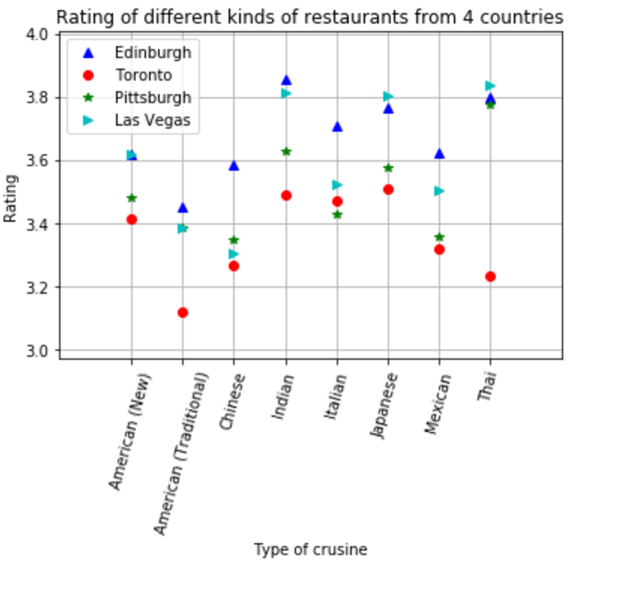
\includegraphics[width=0.4\linewidth]{Rating_different_restaurants_countries}
}
\end{figure}

\section*{3 Data Mining Analysis}

\subsection*{3.1 Geographic Based Clustering}
To find what cuisines may lie in particular neighborhoods in Pittsburgh, we performed two clustering techniques: K-Means and GMM. In order to do this, we decided to look at the closeness and similarities of the restaurants by using the longitude and latitude which considered cluster closeness, as well as the category/cuisines to cluster for similarity. During the data exploration, we intentionally dug into all the types of categories, realizing that we would want to filter out other non-restaurant businesses as well as things such as 'cafe' or 'breakfast' which we didn't identify as a cuisine. This left us with a list of 49 cuisines. We didn't consider any cuisine that had less than 10 restaurants. The SQL data was parsed into a pandas dataframe which has two columns for latitude and longitude, and the remaining are all the cuisines in Pittsburgh. Using the one-hot method, if a restaurant is of that cuisine then the value for the column is 1. To account for the curvature of the earth, though you might want to adjust degrees of longitude and latitude, feature scaling was performed on longitude and latitude in order to scale down the location to a range of cuisines. This was done by subtracting the mean of the whole column from each value, dividing that by the standard deviation in order to get the z-score. We selected 5 to be the appropriate number of clusters for KMeans++ by creating a plot to show the error vs. the number of clusters since it appears to be the greater 'bend' in the elbow.

\begin{center}[h]
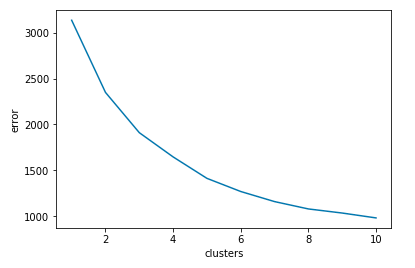
\includegraphics[width=70mm,scale=0.5]{kmeanserror}
\end{center}

With the GMM implementation, we use co-variance as 'spherical' so that each component has its own single variance. As since in the figures below, the longitude/latitude of the restaurants have been plotted and each cluster is labeled with a cuisine. In order to avoid dominance of a particular cuisine purely because the number of restaurants it has in Pittsburgh, we calculated the ratio of each cuisine in the cluster with the total number of restaurants in that category, and then selected the category that has the maximum ratio to be the cluster label.

\begin{center}[h]
	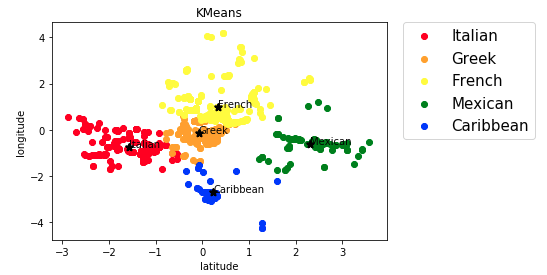
\includegraphics[width=70mm,scale=0.5]{kmeans}
	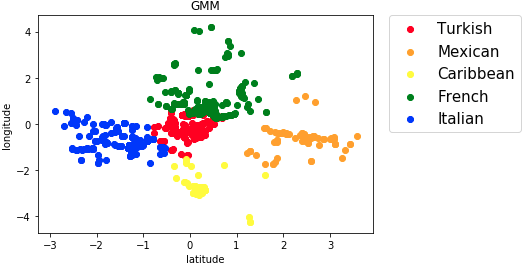
\includegraphics[width=70mm,scale=0.5]{gmm}
\end{center}

\subsection*{3.2 Review-based Recommendation System}
Currently, review analysis is very useful under many recommendation systems scenarios. Specifically, for our project, we are trying to build up a demo of recommendation system based on the reviews for each restaurant. Generally, we are going to build up restaurants profile as well as the user profile based upon text reviews information. For the sake of implementing algorithms, we are going to use tf-idf method to transfer the words vectors to numeric vectors. By matching users’ review profile with the most similar cluster of restaurants, we can build up a simplified review based recommendation system.

\subsubsection*{3.2.1 TF-IDF}
\textbf{TF-IDF} stands for term frequency–inverse document frequency, which is numerical statistic that is intended to reflect how important a word is to a document in a collection or corpus. For our project, we are using TF-IDF as method to turn text data to numeric vector. Basically, TF-IDF is extension of the concept of frequent itemset. \textbf{TF} stands for term frequency, which means the number of times a term occurs in a document. The more frequent one words appear in one document, the more important of this term is for a certain document. \textbf{IDF} stands for the inverse document frequency, which diminishes the weight of terms that occur very frequently in the document set and increases the weight of terms that occur rarely. TF-IDF weight is the product of TF term and the IDF term. Terms with higher TF-IDF scores are better to represent the information of each documents and vice versa.

\subsubsection*{3.2.2 Text Review to Numeric Matrix and Clustering}
Specifically, we extracted all restaurants in Pittsburgh along with reviews from the yelp SQL dataset. We merged all reviews for each restaurant into a single document. By using package NLTK, we preprocessed raw text review data by tokenization, stemming and lemmatization. And then, we build up a dictionary containing all preprocessed words. We wrote our own TF-IDF algorithm and turn text review profile to numeric TFIDF weight profile for each restaurant. After that we implemented K-means clustering algorithm using K-means ++ method offered by sklearn package. The relationship between cluster number and SSE is shown as following graph. However, it seems the SSE is not very good criteria to pick up the K because there is not obvious elbow point on the graph. We will try some other methods to pick up an appreciate number of clusters. 

\begin{center}[h]
	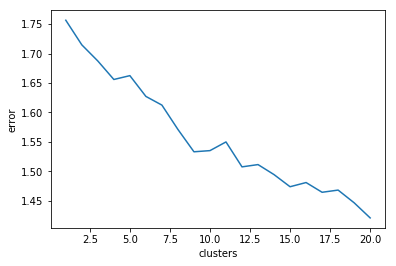
\includegraphics[width=70mm,scale=0.5]{KvsError}
\end{center}

\subsubsection*{3.2.3 Evaluation for Recommendation System Performance}
For the next step, we are going to pick up several sample users to build up the users’ review profile. Try to come up with methods finding out most similar cluster to the user profiles. For the evaluation part, we plan to use our own criteria, which is to check the average rating score of restaurants a user has been to in the clusters. The reviewed analysis improves the performance of recommendation system if the score is above the average score of all restaurants in the cluster and all restaurants the user has been. 
 
\subsection*{3.3 Topic Modeling}

Topic modeling is a text-mining tool for discovery of hidden semantic structures in a text body. It's an Unsupervised Learning Technique that assumes documents are produced from a mixture of topics. The "topics" produced by topic modeling techniques are clusters of similar words. Using contextual clues, topic models can connect words with similar meanings and distinguish between uses of words with multiple meanings. 
Most common topic models are Latent Semantic Indexing (LSI), Latent Dirichlet Allocation (LDA), Hierarchical Dirichlet Process (HDP). The main idea of all these models if find the "abstract" topics that occur in a collection of documents. We chose to use LDA since it is usually preferred the most due to it's better results by using a generative probabilistic model. We will be discussing Latent Dirichlet Allocation (LDA) in detail.

\subsubsection*{Latent Dirichlet Allocation}
Latent Dirichlet allocation (LDA) is a particularly popular method for fitting a topic model. It models each document as dirichlet mixture of topics, and each topic as a mixture of words. This allows documents to “overlap” each other in terms of content, rather than being separated into discrete groups.
This dataset, the restaurants in Pittsburgh which have atleast 200 reviews (there are 109 restaurants and 38,785 that match our criteria), will allow us to extract the latent subtopics and pinpoint areas of interest. We distinguish these reviews as positive reviews and negative reviews based on their rating. Data cleaning of these reviews has to be done carefully or else the algorithm can't perform much because we would be feeding it a lot of noise. So we are including only the terms that occur atleast 10 times in the corpus into the training model because the less frequent terms won't be contributing much to the topic and they increase the size of our document vector that also leads to more training time. We use gensim, a tool for discovering the semantic structure of documents by examining the patterns of words. All our cleaned reviews are fed to LDA model. Here are a word clouds of 8 topics consisting of different words. Note that same word can be present in multiple topics.
Note that we can get any number of topics we want. We set it 8 to get a brief overview of how data looks like. Font in the word cloud indicates the frequency of the word in the topic. Higher the frequency of the word in topic, higher would be the font.

\begin{figure}[h]
\centering
{
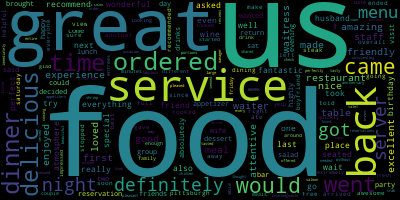
\includegraphics[width=0.4\linewidth]{lda_positive_1}
}
{
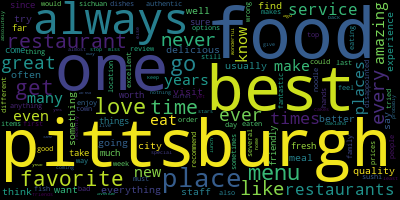
\includegraphics[width=0.4\linewidth]{lda_positive_2}
\vspace{0.1cm}
}
{
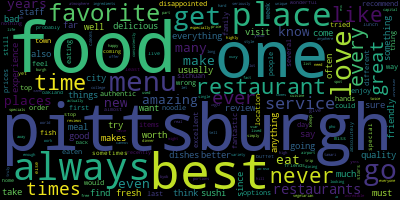
\includegraphics[width=0.4\linewidth]{lda_positive_3}
}
{
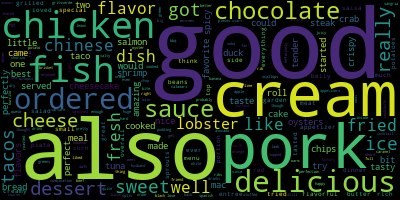
\includegraphics[width=0.4\linewidth]{lda_positive_4}
\vspace{0.1cm}
}
{
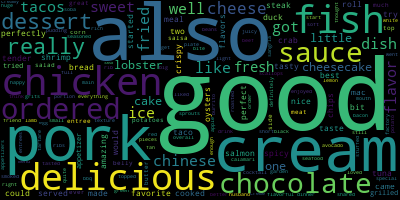
\includegraphics[width=0.4\linewidth]{lda_positive_5}
}
{
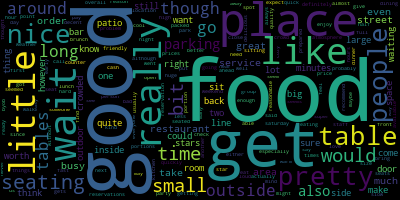
\includegraphics[width=0.4\linewidth]{lda_positive_6}
\vspace{0.1cm}
}
{
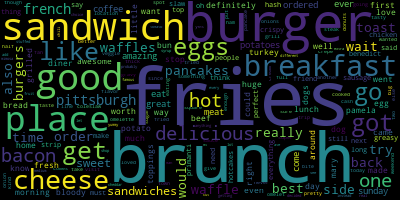
\includegraphics[width=0.4\linewidth]{lda_positive_7}
}
{
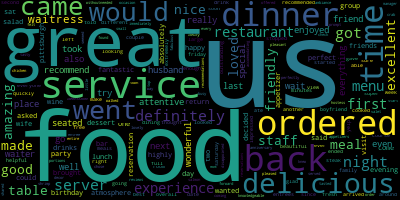
\includegraphics[width=0.4\linewidth]{lda_positive_8}
}
\caption{LDA Positive Results using WordClouds}
\end{figure}


\begin{figure}[h]
\centering
{
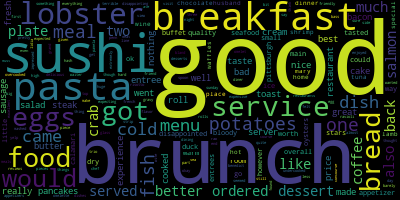
\includegraphics[width=0.4\linewidth]{lda_negative_1}
}
{
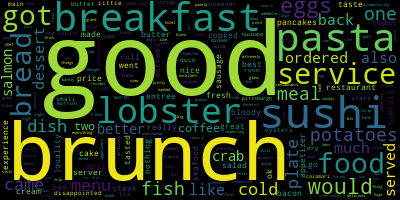
\includegraphics[width=0.4\linewidth]{lda_negative_2}
\vspace{0.1cm}
}
{
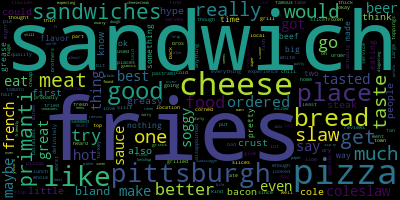
\includegraphics[width=0.4\linewidth]{lda_negative_3}
}
{
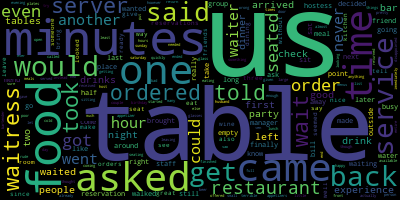
\includegraphics[width=0.4\linewidth]{lda_negative_4}
\vspace{0.1cm}
}
{
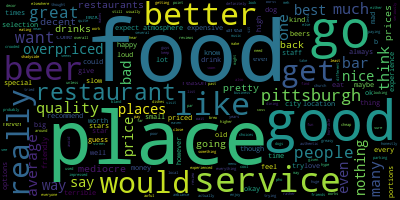
\includegraphics[width=0.4\linewidth]{lda_negative_5}
}
{
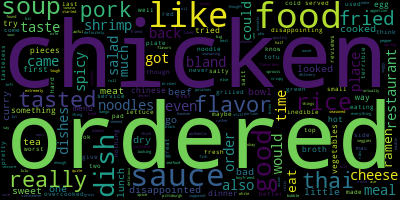
\includegraphics[width=0.4\linewidth]{lda_negative_6}
\vspace{0.1cm}
}
{
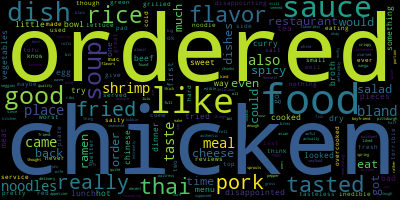
\includegraphics[width=0.4\linewidth]{lda_negative_7}
}
{
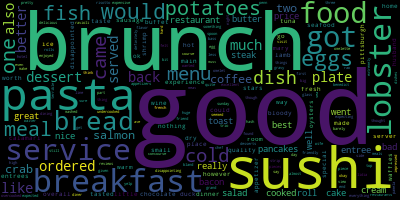
\includegraphics[width=0.4\linewidth]{lda_negative_8}
}
\caption{LDA Negative Results using WordClouds}
\end{figure}

We can observe that words like “place”,“good”,”food”,”chicken” can be observed in almost all the word clouds because we have selected poor number of topics. We can improve this by training the model with more number of latent features (number of topics). With very high number of topics, we need a better tool for exploratory analysis. 
Note that high font size of words like “place”,”good”,”food” in all the wordclouds is due to the very high frequency of these words in their respective topics. If we increase the number of topics, repetition of these words in multiple wordclouds would decrease but fontsize in their respective wordcloud wouldn’t decrease. 

\subsubsection*{Visualization using PyLDAVis}
We will be using pyldavis, a Python LDA Visualization tool for LDA Models. Below is a visual for our lda model on negative reviews with 50 topics. For more detailed exploratory analysis, download this\footnote{\url{https://github.com/emily-jean/yelp-data-mining/blob/master/project/topic-modeling/visualization_negative_50.html}} html page and run it in your browser.

\begin{figure}[h]
\centering
{
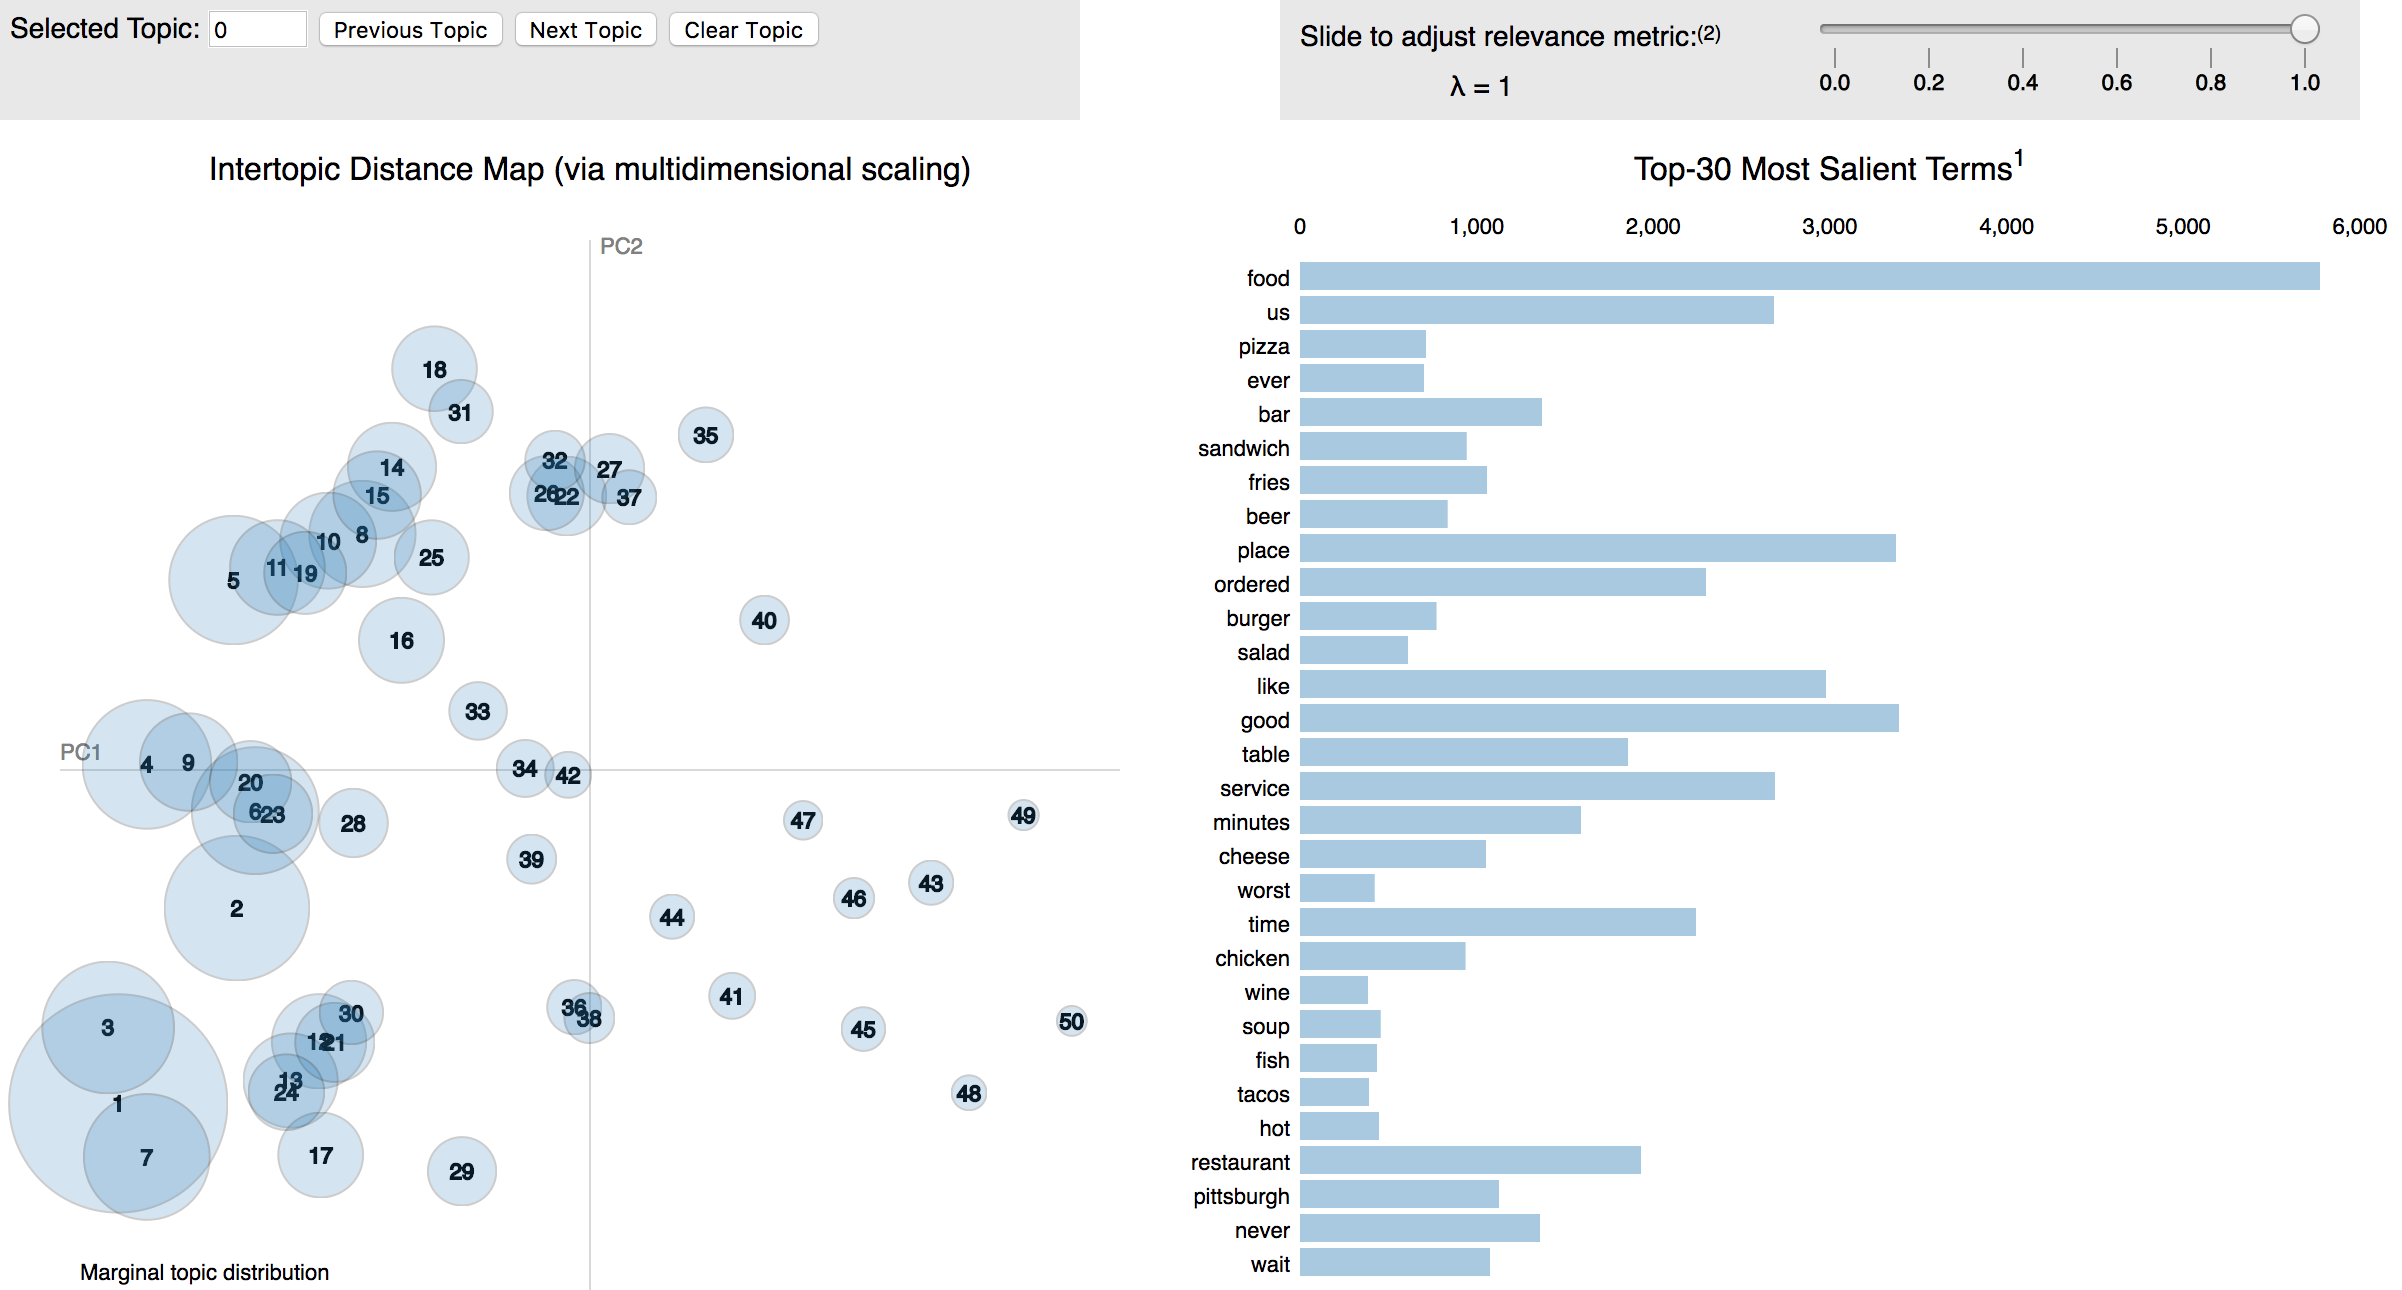
\includegraphics[width=0.4\linewidth]{first_image}
}
\end{figure}

In the above image we have 50 circles representing each topic. Area of the circle represents the prevalence of the topic. The length of the bars on the right represent the membership of a term in a particular topic. In addition to visualizing topic prevalence, the left pane shows inter-topic differences. The distance between topics is calculated using Jenson Shannon Distance, a method of measuring similarity between two probabilistic distributions. (A topic in LDA is a multinomial distribution over the (typically thousands of) terms in the vocabulary of the corpus). It can also be inferred that topics consisting same/similar words would very near to each other.
Each topic’s overall prevalence is encoded using the areas of the circles, where topics are sorted in decreasing order of prevalence. Note the Area of topic 1 > topic 2 > ... Topic50.
Notice what happens when we click on Topic 1. The right panel of our visualization depicts a horizontal barchart whose bars represent the individual terms that are the most useful for interpreting the currently selected topic on the left. Words with high frequency are present in the top of the panel. A pair of overlaid bars in the right panel represent both the corpus-wide frequency of a given term as well as the topic-specific frequency.

\begin{figure}[h]
\centering
{
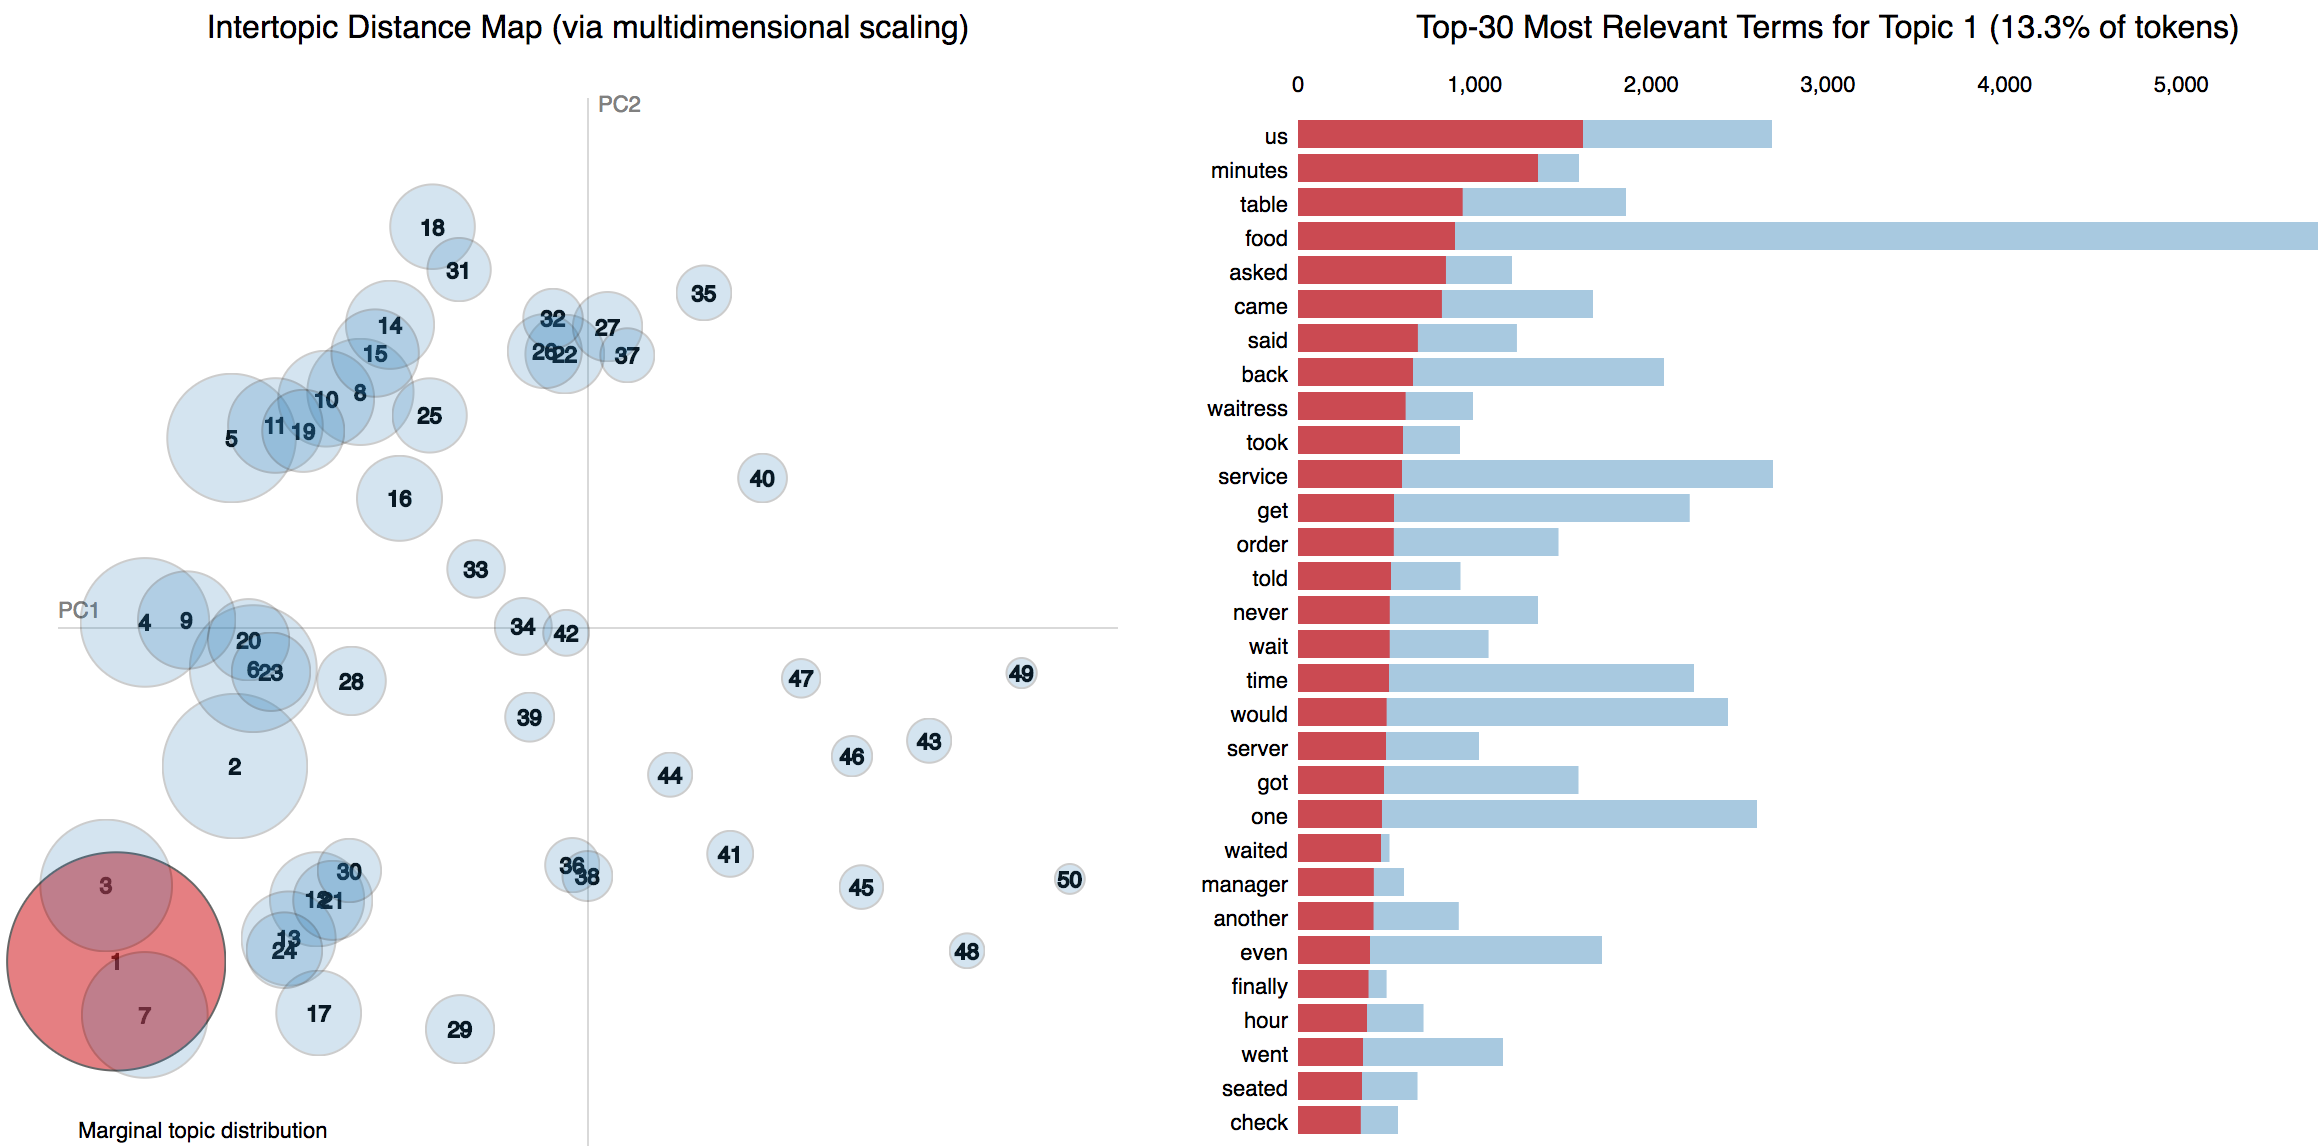
\includegraphics[width=0.4\linewidth]{second_image}
}
{
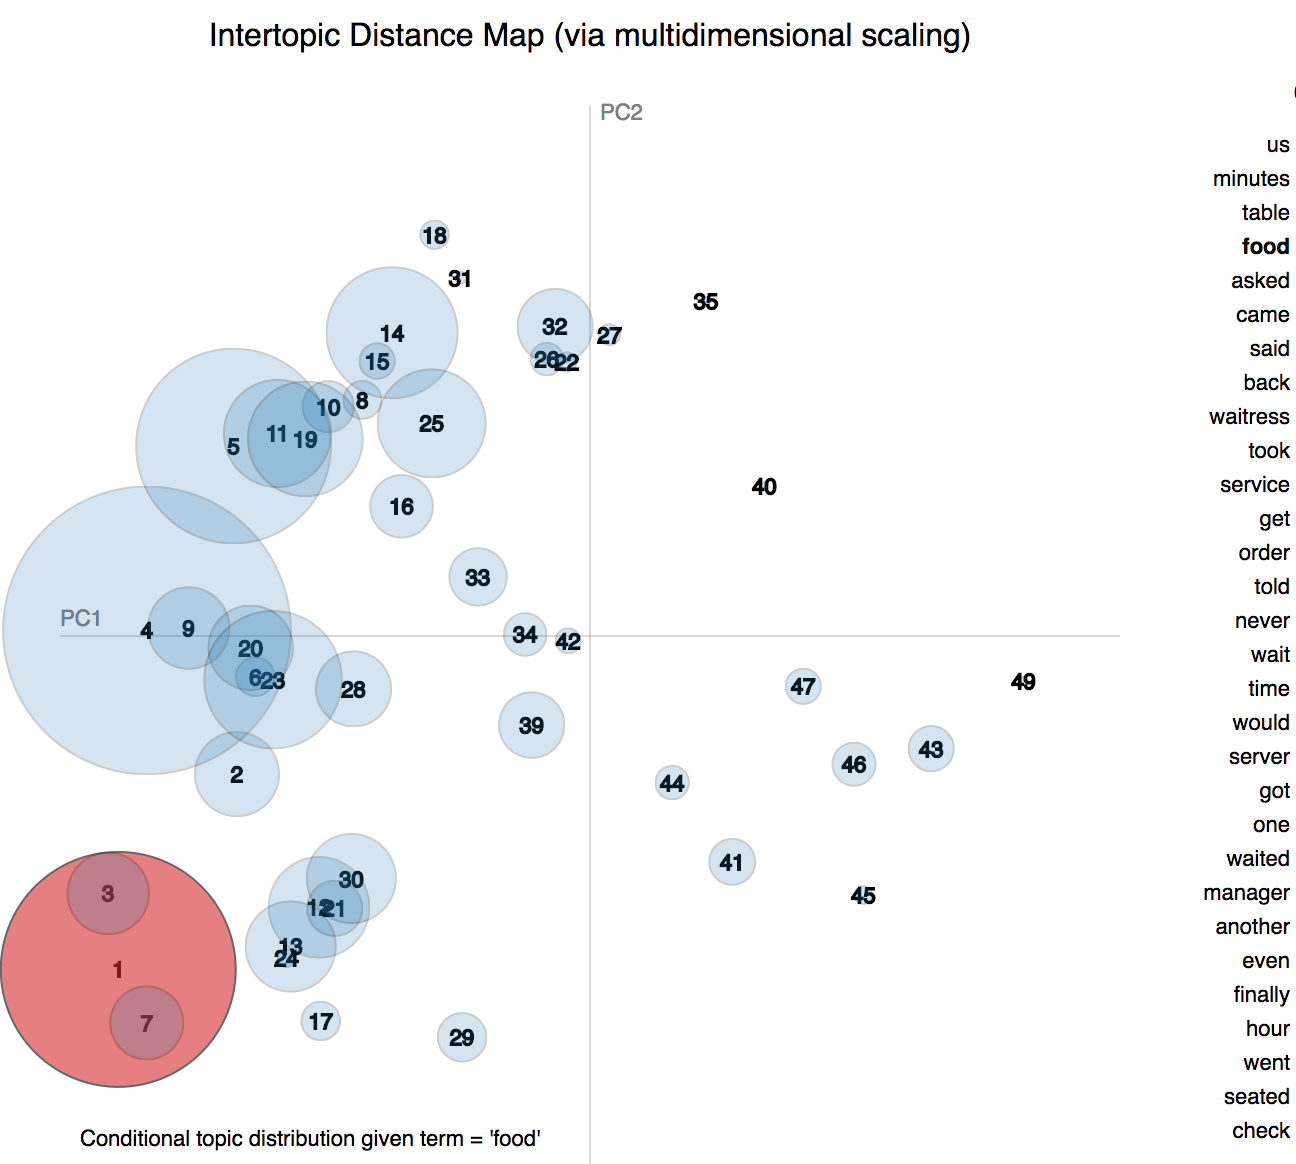
\includegraphics[width=0.4\linewidth]{third_image}
}
\end{figure}

Selecting a term on the right (as shown in the above image)  reveals the conditional distribution over topics (on the left) for the selected term (food). This kind of linked selection allows users to examine a large number of topic-term relationships in a compact manner.
To interpret a topic, one typically examines a ranked list of the most probable terms in that topic, using anywhere from three to thirty terms in the list. The problem with interpreting topics this way is that common terms in the corpus often appear near the top of such lists for multiple topics, making it hard to differentiate the meanings of these topics. So ranking terms for a given topic in terms of both the frequency of the term under that topic as well as the term’s exclusivity to the topic, which accounts for the degree to which it appears in that particular topic to the exclusion of others. We call this relevance of a term to a topic that allows users to flexibly rank terms in order of usefulness for interpreting topics. Setting $\lambda = 1$ results in the familiar ranking of terms in decreasing order of their topic-specific probability, and setting $\lambda = 0$ ranks terms solely by their lift. We learn to set an optimal value of $\lambda = 0.6$ for topic interpretation from a case study.
Let’s us see the most ranked words of topic 1 when $\lambda = 0, \lambda = 0.6$ and $\lambda = 1$.

\begin{figure}[h]
\centering
{
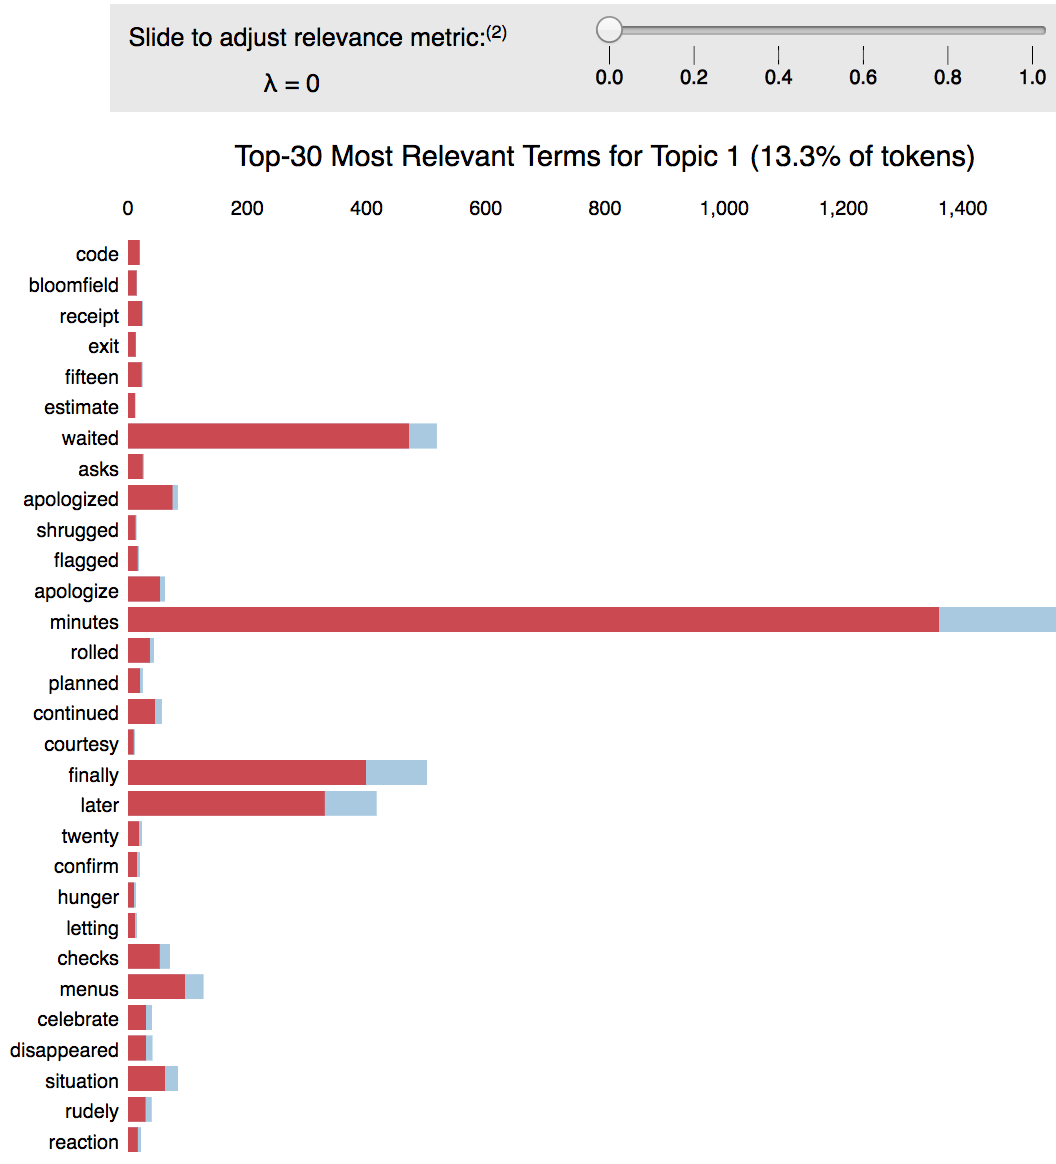
\includegraphics[width=0.4\linewidth]{lambda0}
}
{
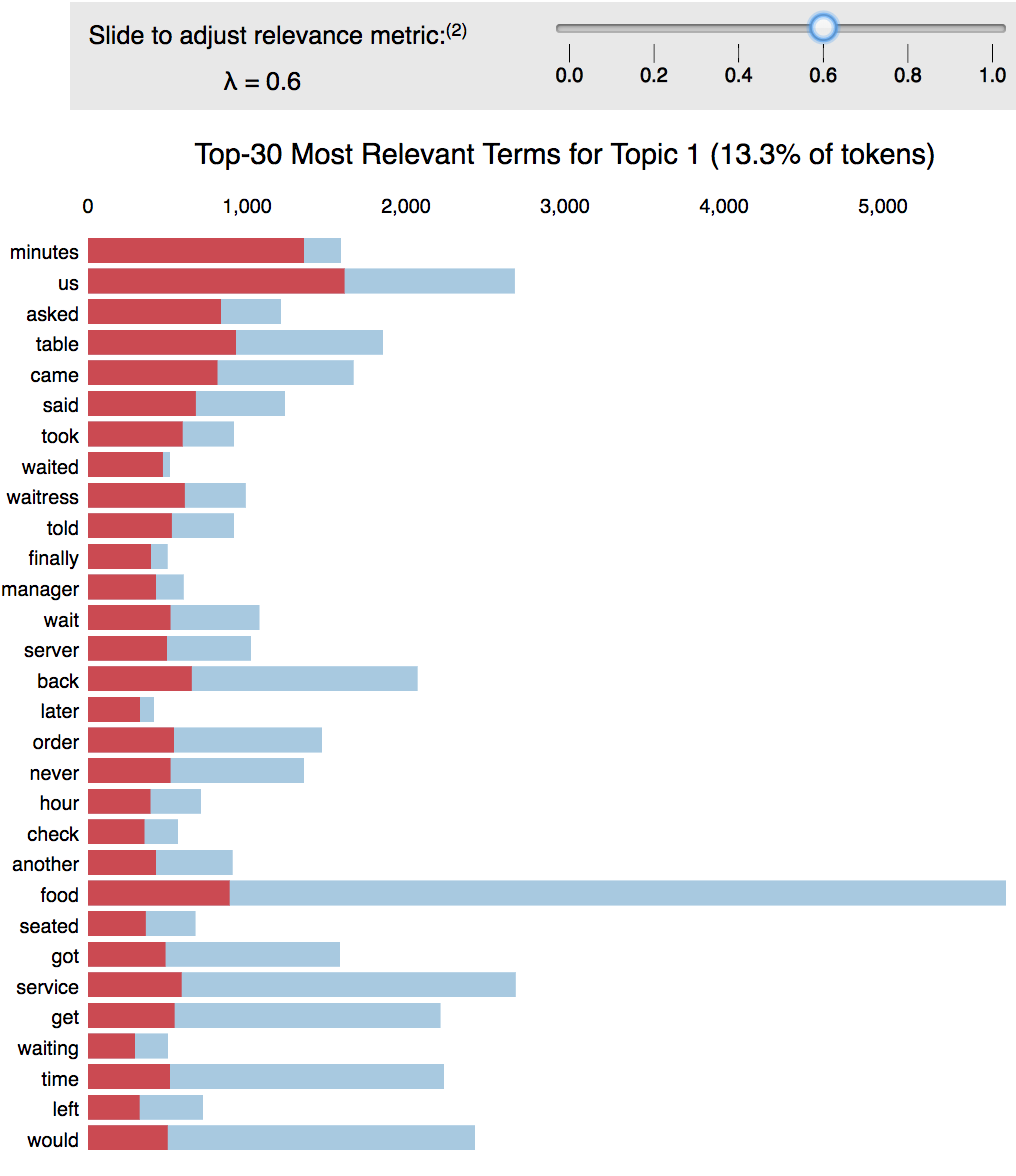
\includegraphics[width=0.4\linewidth]{lambda06}
}
{
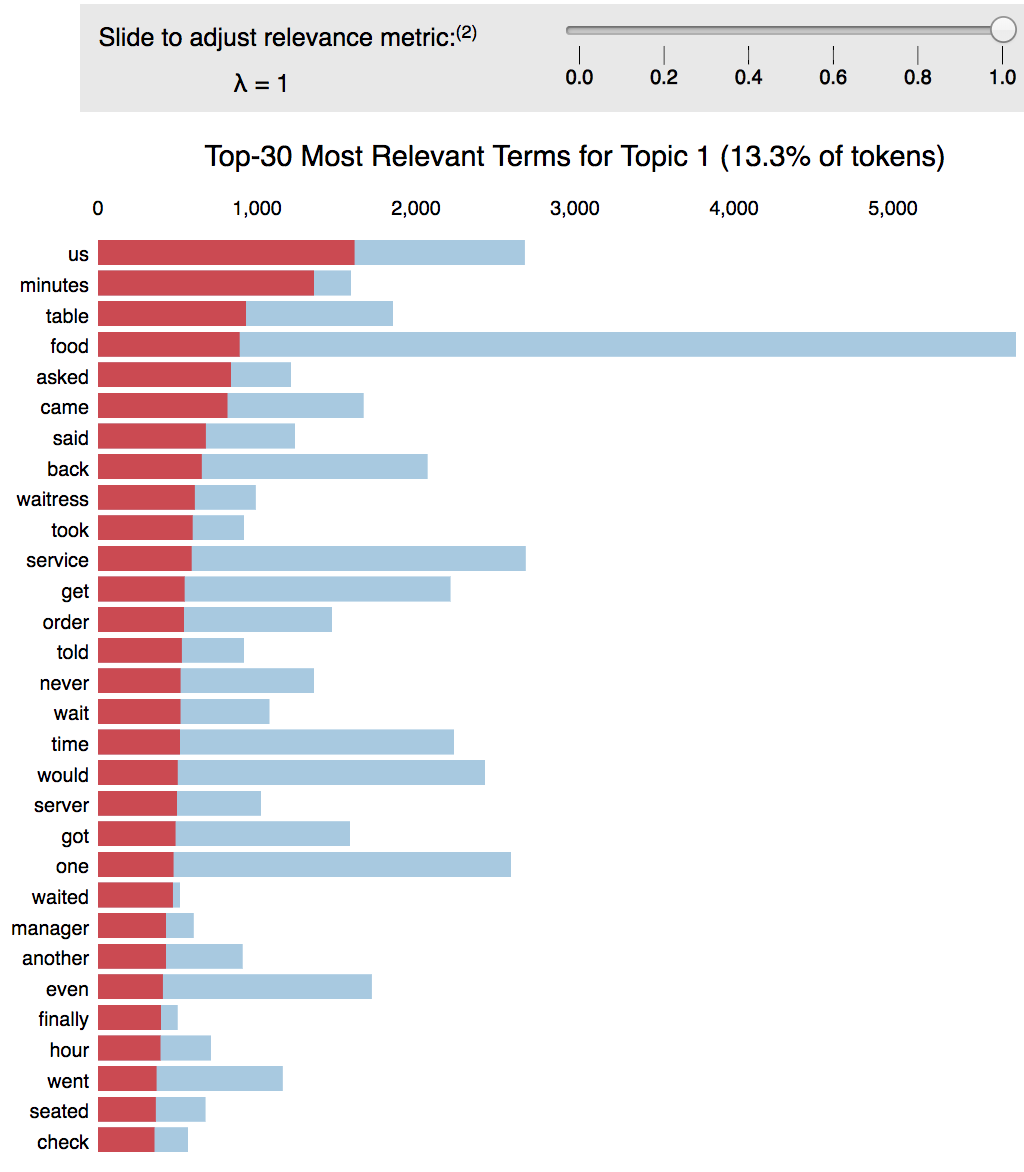
\includegraphics[width=0.4\linewidth]{lambda1}
}
\end{figure}

From above plots it can be clearly observed that when $\lambda = 0$ words that occur only this topic are ranked high. When $\lambda = 1$, words that occur with highest number of times are ranked high. So we choose an optimum $\lambda = 0.6$ for better topic interpretation.
Similar kind of analysis could also be done with positive reviews also. Download this\footnote{\url{https://github.com/emily-jean/yelp-data-mining/blob/master/project/topic-modeling/visualization_positive_50.html}} html page and run it in your browser for data exploration of LDA model on positive reviews with 50 topics. 
Note that number of topics = 50 is still an approximation but a better approximation than 8.  Optimum value of number of topics can be found using Topic Coherence which we would be focusing on in our next report. 
	





\section*{4 Discussion}

Looking at the overall results of our data analysis and implementation, the group was pleasantly surprised by the outcomes.

With our original intention to cluster cuisines by neighborhoods, K-Means had more well-defined clusters since each point only belongs to one cluster. On the other hand, GMM has over-lapping clusters since it calculates the probability of a point belonging to each cluster and therefore seemed to give better clustering.


\section*{5 References}




\end{document}
